




\chapter{Validation of Injection Channel}

Without loss of generality, We injected several binary blackhole signals into PCal to test the performance of our De-Whitening Filter. Unfortunately, at this moment, we couldn't find a compatible data-taking system with desired noise level and dynamical range to faithfully reconstruct or estimate the expect End-Test Mirror (ETM) displacement that caused by our Photon Calibrator. The reason is that the ADC we used has much larger noise than the DAC we used. To beat the ADC noise, although we can amplify the signal before feeding it into the ADC, as what we did for noise measurement in last chapter, some part of injected waveform can easily saturate our ADC. Therefore, the results showed in this chapter should be treated as a demonstration of injecting simulated GW waveforms to PCal. The result should not be used for estimating noise performance.

The injection wavefrom template is generated by IMRPhenomD\footnote{IMRPhenomD is a phenomenological binary blackhole coalescence waveform generating method including both Inspiral, Merger, and Ringdown phase.} code in LALSuite\footnote{LALSuite is the LIGO Scientific Collaboration Algorithm Library Suite}. 
 


  

\begin{figure}[hbt!]
\centering
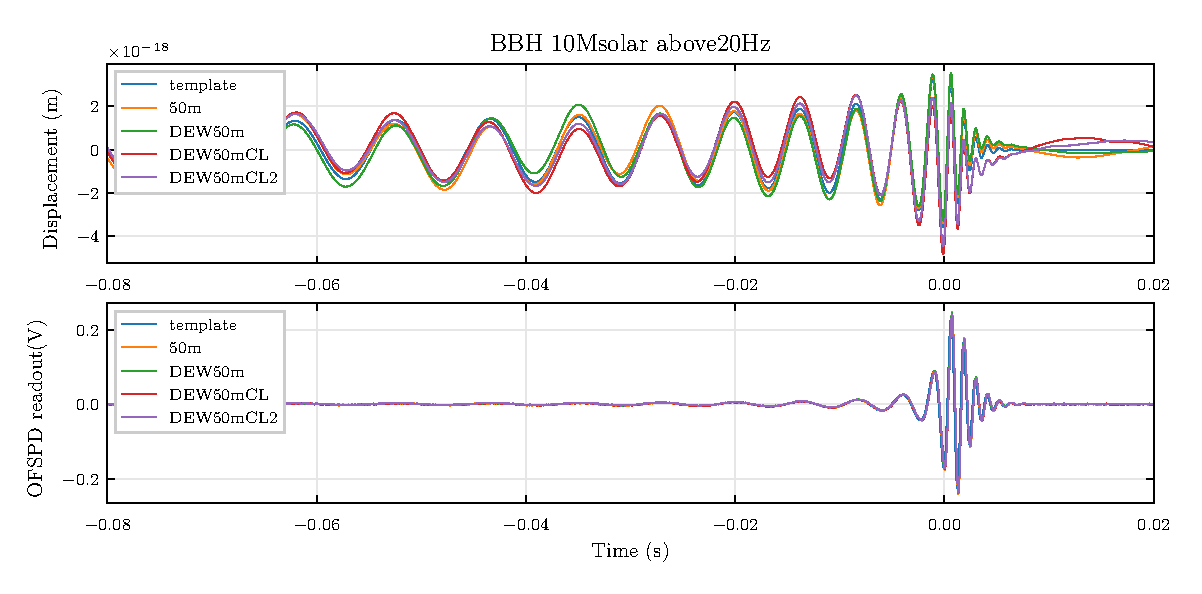
\includegraphics[width=\textwidth]{figure/inj/10.eps}


\includegraphics[width=\textwidth]{figure/inj/20.eps}


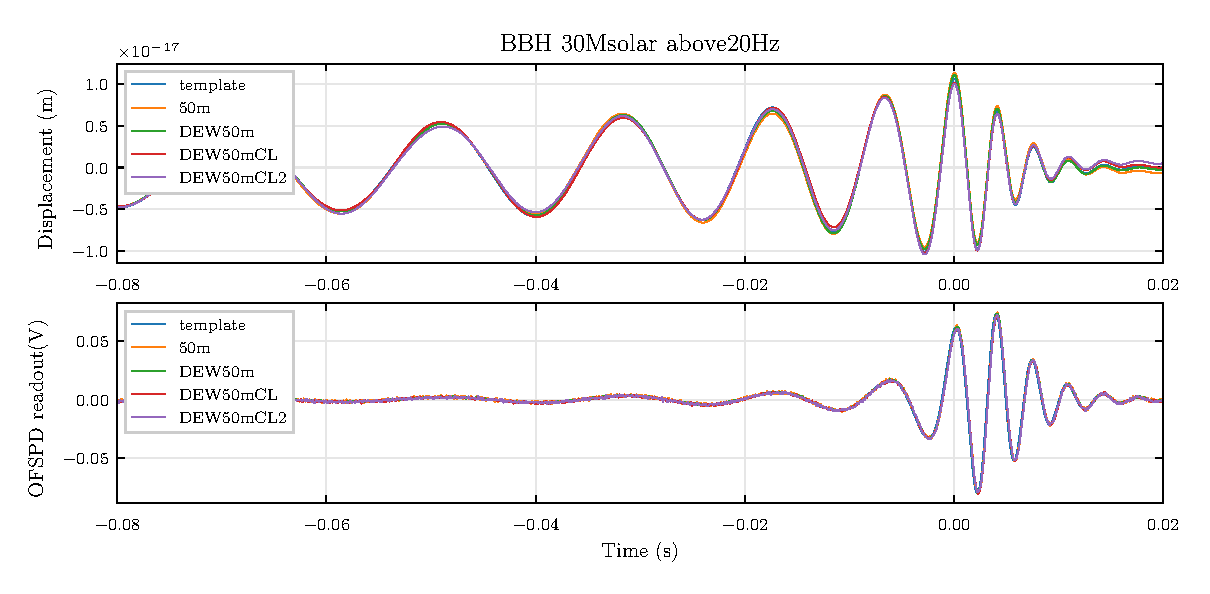
\includegraphics[width=\textwidth]{figure/inj/30.eps}
\caption{Injected Binary Blackhole Merger Signal}\label{fig:bbhinj}
\index{figures}
\end{figure}




